

%************************Document class********************************************
% Define document class with options
% Available font size: 10pt, 11pt, 12pt
% Default options: 11pt, a4paper, onecolumn, onside, final
%************************************************************************************

\documentclass{chart}

%\documentclass[twocolumn]{chart}

% ****************** packages*******************************************************
% following packages are already added 
% ams, xcolor, caption, subcaption, booktabs, footmisc, microtype, graphicx, 
% appendix, geometry, natbib 
%************************************************************************************

%************************Font setting************************************************
% Add the packages at this place
% Default font: `txfonts' which is one of the 'times' fonts
% Remove the below package and add the font package which you like
%************************************************************************************

\usepackage[varg]{txfonts} 

%**************Line spacing, page margins, and graphics*****************************
% Default line spacing for abstract and references is one, and for sections, it is 1.33
% Change line spacing with '\linespacing[]', 
% e.g., \linespacing[1.66] for doublespacing
% Default page margin: top=bottom=left=right= 2 cm   
% Change default margin with the `\geometry' command 
% Graphics path can be set if images are in separate folder
%**********************************************************************************

%\geometry{margin=2.5cm}

\graphicspath{{Images/}}  

%***********************Bibliography********************************************** 
% Default reference style is 'rsc'
% For citation styles, use'\citestyle[options] command
% Available options: numbers, sort&compress, super, square, authoryear, etc.
%*********************************************************************************

%\citestyle[authoryear]

\refstyle{rsc}

%*********************User defined macros/packages********************************
% Define the required newcomands/renewcomands/renewenvironments
% Change abstract color with '\abscolor{backgroundcolor}' command
% Any other document setting
%*********************************************************************************

%\abscolor[linecolor=red]{backgroundcolor=yellow!10} 
%\hypersetup{hidelinks}

%%************************ Details for title page********************************
% Provide the information about title, author, date, email, and address
% Enable \chcopyright[], if you want to suppress the copyright information
%*********************************************************************************

\title{BALANCING EVERYDAY TASKS AND PROJECT MANAGEMENT WITH EASE } 

\author{Akhila Jakamukala}

\date{2023}

\Email{akhilareddy954@gmail.com}

\address{Concordia University, Montreal QC, Canada}

%\chcopyright[] 

%%***************************** Main body*****************************************
% Main body starts from \begin{document} command
%*********************************************************************************

\begin{document} 
	
%==============================Frontmatter=========================================== 
\maketitle    %
%*************%
\begin{abstract}
 Project management is the discipline of planning, organizing, securing, managing, leading, and controlling resources to achieve specific goals. The major challenges of project management include unrealistic deadlines, a lack of communication, unclear dependencies, an inability to manage risk, a lack of unobstructed vision and goals. It is tough to meet these hurdles, and often the project fails due to not meeting these challenges. When project dispersion is higher, the problem is significantly worse. Without the proper guidance, estimating daily effort or reallocating resources can be difficult and causes action from the project lead. Developing effective guidelines, creating an intuitive depiction of the project structure, managing resources and time, and showing more effective dispute resolution strategies are only a few of the difficulties met in resource and project management. Coordination of several project components is necessary for software project management to produce a successful outcome. \\
 	            
\begin{keywords}
 Project management  ,Unclear dependencies ,Reallocating resources ,Prioritization ,Planning,Organizing. 
\end{keywords} 
	
\end{abstract}

\figurespagefalse         
\tablespagefalse           
\makecontents              
 
%================================Mainmatter=========================================
\section{Introduction}\label{sec:intro}  
In today's fast-paced world, managing daily tasks while simultaneously handling project-related tasks is a crucial skill. However, the balancing act between routine tasks and project work often results in a decrease in productivity due to a lack of proper time management, prioritization, and strategic planning. There is a need for effective task management strategies that can help individuals and organizations achieve their goals without compromising on either daily operations or project completion. 
\subsection{Motivation} 
Motivation for investigating how to handle day-to-day tasks along with projects is rooted in the recognition of the significant impact that effective time management and project integration can have on individual and organizational success. Efficiently managing daily tasks and projects ensures optimal productivity for individuals and teams. Improved productivity contributes to the overall success and competitiveness of an organization. Ensuring that day-to-day tasks and projects align with organizational strategies is vital for long-term success. Addressing challenges in managing tasks and projects positions an organization as more agile and responsive in the marketplace. Individuals can enhance their skills and capabilities by mastering the art of balancing daily tasks and project responsibilities. Personal and professional development contributes to career advancement and job satisfaction.

\subsection{Problem Statement} 
The problem being investigated is the challenge of effectively managing daily tasks with project responsibilities, focusing on individual and organizational productivity, project success, and overall well-being. Precision in addressing this problem is crucial to ensure a clear understanding of the specific issues at hand. This problem statement aims to provide a precise understanding of the challenges and opportunities associated with handling day-to-day tasks along with project management responsibilities. The investigation seeks to offer insights into practical solutions that promote productivity, work-life balance, and successful project outcomes.

\subsection{Objectives} 
To understand the dynamics of balancing day-to-day tasks along with project work, identifying the common challenges faced by individuals and organizations in managing day to day tasks and projects and to analyze the effectiveness of various task and project management strategies, tools, and methodologies currently in use ,to develop a comprehensive, adaptable, and scalable framework that can assist individuals and teams in managing daily tasks while also handling project work without compromising efficiency and productivity ,to provide actionable insights and recommendations that can enhance individual productivity, team collaboration, and overall organizational performance and also to assess the impact of proposed strategies on stress levels, job satisfaction, and work-life balance of individuals handling both day-to-day tasks and project work.


\subsection{Managing  tasks} 

\subsubsection{Project Management}
A project is a temporary endeavour with a defined beginning and end, undertaken to meet unique goals and objectives, typically to bring about beneficial change or added value. Project management involves the application of knowledge, skills, tools, and techniques to project activities to meet project requirements.Key aspects of project management include planning, organizing, controlling ,leading ,managing ,securing.Effective project management is crucial for delivering projects on time, within budget, and with the expected level of quality. Various methodologies and frameworks, such as Agile, Scrum, and Waterfall, are employed in project management to provide structured approaches to diverse types of projects.~\cref{fig:project management} 
 
\begin{figure}
	\centering
	\includegraphics[width=0.45\linewidth]{Fig1}
	\caption{Prioritizing tasks based on their dependency and urgency} 
	\label{fig:project management}
\end{figure}

\subsubsection{ Managing day-to-day task}
Handling day-to-day tasks along with managing a project can be challenging, but effective time management and prioritization can make the process smoother. “Prioritization is a powerful skill that will help you take control of your workflow and optimize productivity.” Breaking your workload into manageable chunks and setting priorities helps you break the cycle of missed deadlines, last-minute rushes, and procrastination. ~\cref{fig:task management} While all the steps in prioritizing tasks are crucial, the most critical step is understanding how each task ranks in relation to your goals and objectives. By assessing the significance of tasks, you can prioritize effectively and ensure your efforts are directed toward activities that align with your overarching priorities.
 
\begin{figure}
	\centering
	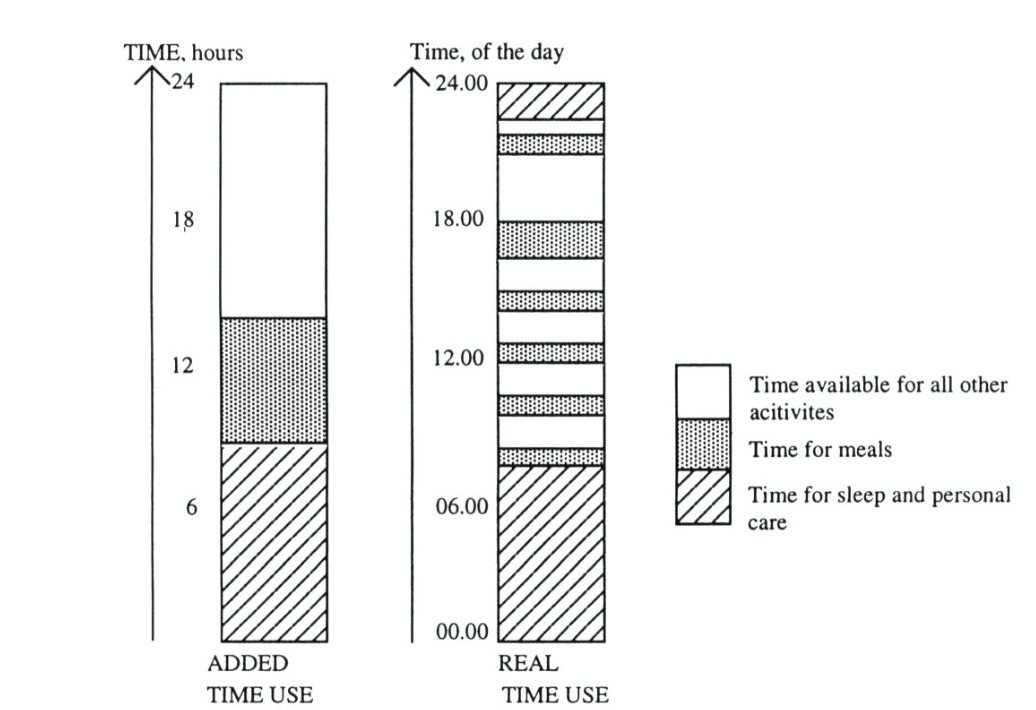
\includegraphics[width=0.45\linewidth]{fig2}
	\caption{Principal difference between added (left) and real (right) time-use.} 
	\label{fig:task management}
\end{figure}

\section{Methodologies} 
\subsection{Time-geographical approach to the study of everyday life contexts} 
Time-geographical approach to the study of everyday life contexts: capturing contexts, grasping totality at the individual level People engage in the factual creation of various contexts when they go about their daily lives. These contexts are all derived from the totality of the activities people go about in their social and geographical settings.In this time-geographical method, the activities of
'living one's life' are described by the basic structure of the hierarchical scheme of categories presented below .~\cref{fig:Activity categorization scheme.} The scheme presented is a foundation for organizing and analyzing the numerous activities in everyday life at both individual and household levels. The time-geographic methodological framework encompasses four contexts: everyday, project, social, and geographical. The everyday context illustrates an individual's activity sequence over time, the project context links activities to personal goals, the social context considers interactions between individuals, and the geographical context locates activities in specific places. Together, these contexts reveal the culture of a society and individual preferences, emphasizing the interconnectedness of activities, goals, social interactions, and physical locations.
\begin{figure}
	\centering
	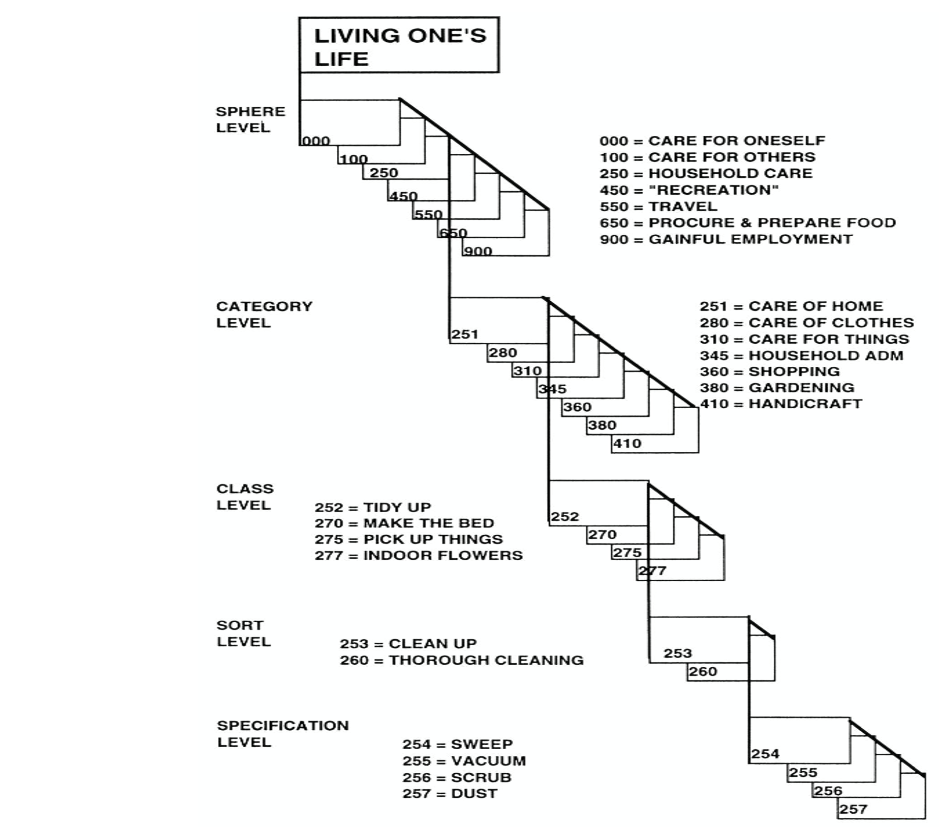
\includegraphics[width=0.45\linewidth]{fig3}
	\caption{Here is an example of how the line from the sphere household care is organized into levels, with some alternatives at each level.} 
	\label{fig:Activity categorization scheme.}
\end{figure}
\subsubsection{ The everyday context}
The everyday context has an underlying structure shaped by the individual's rhythm of physiologically necessary activities and societal timetables (e.g., working hours, shopping hours). The real-time use concept illustrates the principle of the everyday context. For instance, a daily activity sequence might include waking up, work, meals, and sleep. The everyday context is not random but follows a structured pattern. The example of a parent's daily activities prompts questions about the roles of other family members, broader social contexts, and the shared responsibilities within the household. This leads to a discussion of the social context.
\subsubsection{ The project context}
A project context is a configuration of diverse activities related to a particular aim, encompassing both strenuous and enjoyable tasks. Unlike a sequential chain, activities in a project context may be interrupted by activities from other project contexts. This concept is valuable for studying household division of labor, as not all activities within a project context are assigned to specific individuals, providing flexibility in task allocation. For instance, either parent or someone else may perform certain activities, but consistency in performing specific tasks builds trust with those involved. It's recognized that essential project contexts are subject to interruptions from activities in other contexts.
\subsubsection{ The social context}
Analyzing the social context aids in understanding household division of labor strategies, distinguishing between specialization (distinct roles) and cooperation (shared responsibilities). The social context reveals whether household members collaborate or perform tasks in isolation, providing insights into their group dynamics. This context illustrates how people meet in everyday life, aligning activities with individual wants and adjusting to social constraints. Additionally, all activities have a physical location, and the geographical context analyzes where activities occur, considering tools and materials needed.
\subsubsection{ The geographical context}
Developing the geographical context within the time-geographic method involves considering geographical distances and refining location and movement time considerations. Overall, there is ongoing intellectual work to fully develop and sensitize the geographical context within this framework.At the individual level, a rhythmic pattern emerges, emphasizing the significance of the dwelling, workplace, and locations of friends, relatives, and shops. While geographical movement routines vary between households in different countries, the central role of places where friends and relatives live remains consistent.


 \section{Conclusions}
In conclusion, the research highlights the complexities of managing day-to-day tasks along with projects and provides valuable insights into conditions influencing success. While the findings offer practical recommendations for various contexts, the study acknowledges limitations and suggests areas for further refinement. The integration of suggested improvements and a continued exploration of the nuances in diverse organizational settings will contribute to the ongoing evolution of effective strategies in this dynamic landscape.





%***********************************References*********************************	 

\bibliography{References}
 
\end{document}
%%%%%%%%%%%%%%%%%%%%%%%%%%%%%%%%%%%%%%%%%%%%%%%%%%%%%%%%%%%%%%%%%%%%%%%%%%%%%%%%%%% 










